% controlled fusion and RF heating and current drive
%\chaptertoc{}

\chapter{Controlled Fusion, RF heating and Current Drive}
\label{chap:fusion_and_rf}
\margintoc

%%%%%%%%%%%%%%%%%%%%%%%%%%%%%%%%%%%%%%%%%%
%%%%%%%%%%%%%%%%%%%%%%%%%%%%%%%%%%%%%%%%%%
\section{Nuclear Fusion}
Nuclear fusion is the process that powers all the stars in the Universe, including our Sun. To get nuclear fusion, nuclei have to come close enough to each other where nuclear forces can overcome their mutual electrostatic repulsion. This would require temperatures of the order of 720 keV for head-on collisions of thermal particles to lead to fusion reactions in a classical way. 

Actually, quantum physics has to be taken into account in the process. Both in tokamaks and in stars interiors, fusion reactions take place predominantly due to the tunnel effect. Crossing this barrier can be quantified in a probabilistic manner with the reaction rate $R$ $[\mathrm{reaction/m^3 s}]$, defined as the probability of reaction per unit time and volume. 
The reaction rate between mono-energetic ions of density $n_1$ $[\si{m}^{-3}]$ striking target ions of density $n_2$ $[\si{m}^{-3}]$ is proportional to the effective cross-section area $\sigma$ $[\si{m}^2]$ and to the velocity difference $v_{12}$ between the two species:
\begin{equation*}
	r_{12} = n_1 n_2 \; \sigma v_{12}
\end{equation*}
The quantity  $\sigma v_{12}$, which depends on the kinetic energy of the colliding particles, is called the reactivity ($\mathrm{[m^3/s]}$). The reaction rate $r_{12}$ is proportional to the square of the density of the mixture. In fusion plasmas, ions are not mono-energetic. They are assumed to have Maxwellian velocity distributions. The average reactivity $\langle \sigma v \rangle_{12}$ derives from the following expression:
\begin{equation*}
	\left < \sigma v \right >_{12} 
	= \int_{-\infty}^{+\infty} \int_{-\infty}^{+\infty} 
	\sigma(v_{12}) v_{12}\;  f_1(v_1) f_2(v_2) \; dv_1dv_2
\end{equation*}

Finally, the average reaction rate $R_{12}$ reads:
\begin{equation*}
	R_{12} = n_1 n_2 \; \left < \sigma v \right >_{12}
\end{equation*}
It governs the time evolution of both densities: $\dv{n_1}{t} = \dv{n_2}{t} = - R_{12}$. The temperature dependence of the reactivity $\langle \sigma v \rangle_{12}$ is plotted on figure \ref{fig:chap1:reactivity} for several fusion reactions.

\begin{figure} 
	\begin{center}
		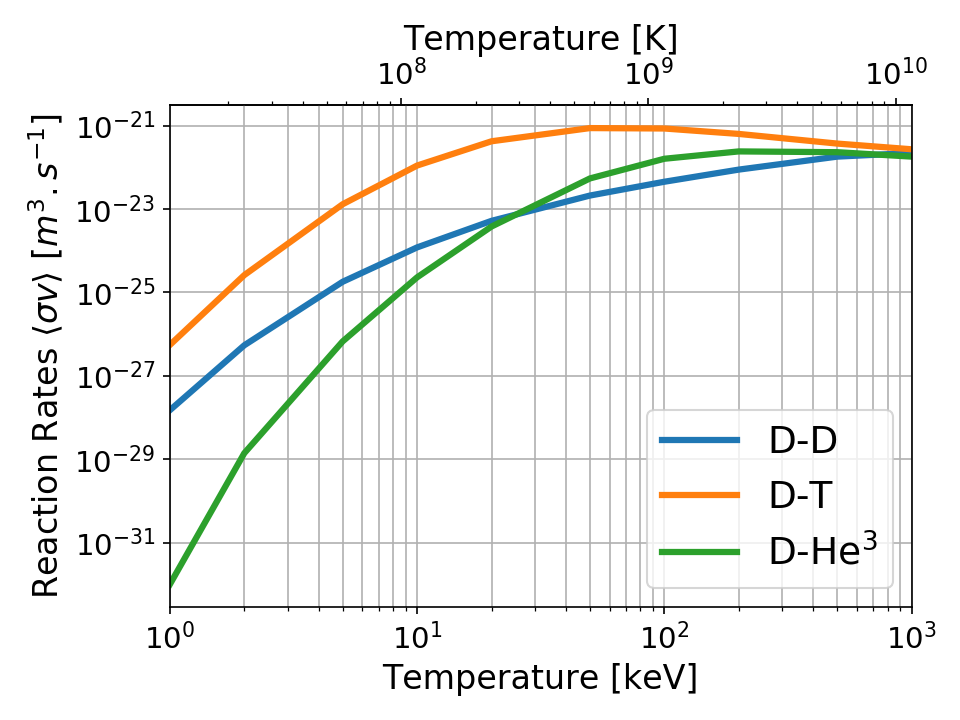
\includegraphics[width=1.0\textwidth]{figures/chap1/Fusion_Reactivity.png}
		\caption{Fusion reactivity versus temperature for few couples of fusion reactions. Data from \citeauthyear{richardson2019}.}
		\label{fig:chap1:reactivity}
	\end{center}
\end{figure}

The D-T reactivity reaches its maximum for a temperature of 64 keV, corresponding to a temperature of $742\,10^6$ K. Since it has the highest reaction rate, the D-T reaction is the “easiest” to initiate (maximum reactivity at lowest temperature) of all fusion reactions and is the main targeted reaction for controlled fusion reactors\sidecite{cea1987, ball2019}: 
\begin{equation}
	\mathrm{D + T} \longrightarrow \mathrm{{}^4 He~(3.56~MeV) + n~(14.03~MeV)}
\end{equation}
Therefore, the D-T reaction leads to a total released energy of $E_{DT}$ = 17.59 \si{MeV} = $2.82\times 10^{-12} \si{J}$ per fusion reaction\sidenote{This value can be compared to the 200~MeV released by $^{235}$U fission. Yet, the energy release \emph{per nucleon} ($i.e.$ per kilogram) is approximately 4 times larger for fusion than for fission reactions.}.

The fusion power per unit volume $p_{DT}$ produced by the fusion of the nuclei of deuterium and tritium reads: 
\begin{equation*}
	P_{fus} = n_D n_T \left< \sigma v \right>_{DT} E_{DT}
\end{equation*}
with $n_D$ and $n_T$ the deuterium and tritium density and $\left< \sigma v \right>_{DT}$ the D-T reactivity. 


The fusion power per unit volume $p_{DT}$ produced by the fusion of the nuclei of deuterium and tritium reads: 
\begin{equation*}
p_{DT} = n_D n_T \left< \sigma v \right>_{DT} E_{DT}
\end{equation*}
with $n_D$ and $n_T$ the deuterium and tritium density and $\left< \sigma v \right>_{DT}$ the D-T reactivity. Assuming equal deuterium and tritium densities:
\begin{equation*}
n_D = n_T = \frac{n}{2}
\end{equation*}
with $n$ the electron density, then the thermonuclear power density is:
\begin{equation*}
p_{DT} = \frac{1}{4} n^2 \left< \sigma v \right>_{DT} E_{DT}
\end{equation*}

%Assuming a constant reactivity in the plasma ("flat profile hypothesis") and using the tore volume $V$, the fusion power is: 
%\begin{equation}
%P_{fus} = \frac{V}{4}
%n^2 \left< \sigma v \right>_{DT} E_{DT}
%\end{equation}
%
%For a circular cross-section, the plasma volume is $V=2\pi^2 R a^2$. The reactivity $\left< \sigma v \right>_{DT}$ depends on the temperature. In the temperature range 10.3-18.5 keV, it turns out that the reactivity $\left< \sigma v \right>_{DT}$ can well (with about 10$\%$ error) be approximated by \sidecite{wesson2011}: 
%\begin{equation*}
%	\left< \sigma v \right>_{DT} \approx 1.18\, 10^{-24}\; \hat T^2 \;\si{\left[m^3 s^{-1}\right]}
%\end{equation*}
%where $\hat T$ is expressed in $\si{keV}$.

%%%%%%%%%%%%%%%%%%%%%%%%%%%%%%%%%%%%%%%%%%
\section{Magnetic Controlled Fusion}
If controlled in a reactor, fusion power could be an ideal energy source. It would run on hydrogen isotopes\sidenote{Such as deuterium which can be found in sea water and tritium which can be generated inside the reactor}, does not generate greenhouse gas and creates no radioactive waste except the reactor vessel components itself. It would be dispatchable source (in contrast to intermittency inherently affecting solar and wind energies) and would require much less land area than wind or solar power installations for similar power. But producing a self-sustaining fusion reaction requires that deuterium and tritium be heated to over 150 million K, a temperature at which they become plasma: an electrically charged gas. 


Sustaining a high temperature in steady-state requires that the plasma be confined by magnetic field.

\section{Tokamak}
The magnetic device called \emph{tokamak}, first developed in the Soviet Union in the early 1960s, is an efficient way to confine high temperature plasmas\sidecite{shafranov2001, azizov2012, mirnov2019}. It is an axially symmetric field configuration with a large toroidal magnetic field, a moderate plasma pressure and a relatively small toroidal current\sidecite[+0.4cm]{Freidberg2007}. By virtue of the highest achieved values of the $n T \tau_e$ product, tokamak is presently the leading magnetic configuration for a fusion reactor. Because of its performance, there is a large number of experimental tokamaks currently in operation or being constructed\marginnote{See \href{http://www.tokamak.info/}{www.tokamak.info} for an updated list of past, present and future experiments}. The following machines are cited in this manuscript: WEST (previously Tore-Supra, Cadarache, France), JET (Culham, UK), ASDEX-Upgrade (Garching, Germany), EAST (Hefei, China), HL-2A (Chengdu, China), KSTAR (Deajon, Korea) and the international project ITER (Cadarache, France).

\begin{marginfigure}[0cm]
	
\includegraphics[width=1\linewidth]{figures/chap1/tokamak_toroidal_field}
	\caption{Toroidal magnetic field produced by toroidal field coils.}
	\label{fig:tokamak_toroidal_field}
\end{marginfigure}

\begin{marginfigure}[0cm]
	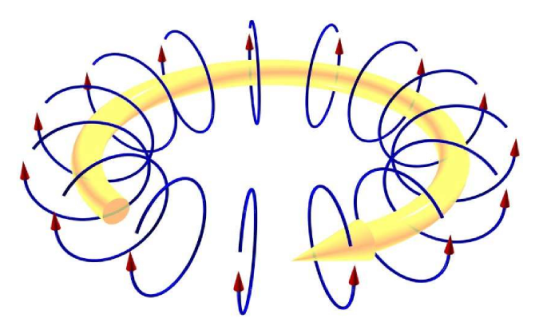
\includegraphics[width=1\linewidth]{figures/chap1/tokamak_poloidal_field}
	\caption{Poloidal magnetic field produced by the plasma current.}
	\label{fig:tokamak_poloidal_field}
\end{marginfigure}

\begin{marginfigure}[0cm]
	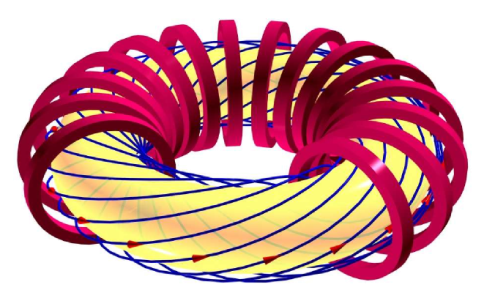
\includegraphics[width=1\linewidth]{figures/chap1/tokamak_helical_field}
	\caption{Helical magnetic field produced by the combination of toroidal and poloidal fields.}
	\label{fig:tokamak_helical_field}
\end{marginfigure}

In a tokamak, the plasma is confined by the combination of two magnetic fields: the toroidal and the poloidal fields. The toroidal field is the strongest one and is created in the toroidal direction by external "toroidal" field coils (Fig.\ref{fig:tokamak_toroidal_field}). Another set  of  external  coils, the poloidal field coils, which includes the central solenoid coils and additional control coils, are located concentric with the toroidal vacuum vessel.

An electric field in the toroidal direction is induced through the plasma by ramping a current in the central solenoid, like an electrical transformer in which the plasma acts as the secondary winding. This electric field induces a current in the plasma, current which creates the poloidal field (Fig.\ref{fig:tokamak_poloidal_field}). Poloidal and toroidal add up to form a twisted helical field (Fig.\ref{fig:tokamak_helical_field}) and both are required to confine the plasma into the vacuum vessel. 


\section{Ohmic Heating and Current Drive}
\subsection{The Need for Additional Heating}

%In a tokamak, a toroidal plasma current is induced by the central solenoid coil. This is called "inductive current drive". 
The plasma current density $J_p$ $\si{A/m^2}$ flowing through plasma with resistivity $\eta$ $\si{\Omega.m}$ heats up the plasma and generates an Ohmic heating power density $p_\Omega$:

\begin{equation}\label{eq:ohmic_power_density}
p_\Omega = \eta \; J_p^2 \;\; \si{[W/m^3]}
\end{equation}

where $\eta$ is the classical (parallel) Spitzer resistivity \cite[Eq.(11.15)]{Freidberg2007}:

\begin{equation}\label{eq:Spitzer_resistivity}
\eta
%= 0.51 \frac{\sqrt{2} e^2 m_e^{1/2} }{12 \pi^{3/2} \varepsilon_0^2 T_e^{3/2}} \ln \Lambda
\approx
3.3 \times 10^{-8} / \hat T^{3/2}  \, \mathrm{\Omega.m}
\end{equation}
\marginnote{$\hat T$ is expressed in \si{keV}: $\hat T=10^{-3} k_B T_{[K]}/e$}

Assuming homogeneous temperature in the plasma volume $V$, the Ohmic power $P_\Omega$ is:

\begin{equation}\label{eq:ohmic_power}
P_\Omega
=
3.3 \times 10^{-8} \frac{ I_p^2 }{ \hat T^{3/2} } V
\end{equation}

Since $\eta$ is proportional to $\hat T^{-3/2}$, $\eta$ decreases with increasing temperature and the role played by the Ohmic heating (\ref{eq:ohmic_power}) gradually becomes less important. 

\marginnote{This section is taken from the "Tokamak dimensioning" activity given to French Master students in the frame of the "Master Fusion" and published in \citeauthyear{sarazin2019}.}
The maximum temperature achievable using only Ohmic heating can be deduced from a 0D approximation by equalling Ohmic power input and losses. The plasma thermal losses, either by collisional conduction or by turbulent convection, is summarized as $P_{\mathrm{th}}$ is:

\begin{equation}\label{eq:plasma_thermal_losses}
P_{th} = \frac{W}{\tau_e}
\end{equation}

where $W$ is the plasma energy is and $\tau_e$ the plasma confinement time, defined as the characteristic time at which the plasma energy is lost by thermal mechanisms. Assuming homogeneous and equal density and temperature between ions and electrons, the plasma energy reads: 

\begin{equation}\label{eq:plasma_energy}
W 
= \int \frac{3}{2} k_B (n_e T_e + n_i T_i) dV 
\approx 3 n k_B T V
\end{equation}

The confinement time $\tau_e$ in L-mode (relevant mode here) can be expressed from its scaling law \cite[Eq.(14.155)]{Freidberg2007}:

\begin{equation}\label{eq:tau_e_modeL}
\tau_{e,L}
=
0.048  I_p^{0.85} R^{1.2} \kappa^{0.5} \hat n^{0.1} B^{0.2} A^{0.5} P_\Omega^{-0.5}
\end{equation}  
%which can be reexpressed as:
%$$
%\tau_L
%=
%0.037  
%\frac{\varepsilon^{0.3}}{q_\star^{1.7}}
%\frac{a^{1.7} \kappa^{1.7} \hat B^{2.1} A}{n_{20}^{0.8} T_k}  
%$$

At equilibrium, Ohmic power balances thermal losses\sidenote{Radiation losses are neglected here.} and the Figure \ref{fig:ohmicpowervsthermallosses} shows that for typical tokamak fusion reactor parameters\sidenote{Main dimensions used:
\begin{itemize}
	\item $a$ = 2 m
	%\item $\varepsilon$ = 0.4
	\item $\kappa$ = 2
	\item $B$ = 4.7 T
	\item $n_{20}$ = 1.5 [$\times 10^{20}$ $\si{m^{-3}}$]
	%\item $q_\star$ = 2
	\item $A$ = 2.5 (average mass number DT mixture)
\end{itemize}
}
the maximum temperature achievable by ohmic heating is about few keV only. This temperature is not high enough for the alpha power to dominate: some other form of external heating is thus required. 

\begin{figure}[h]
	\centering
	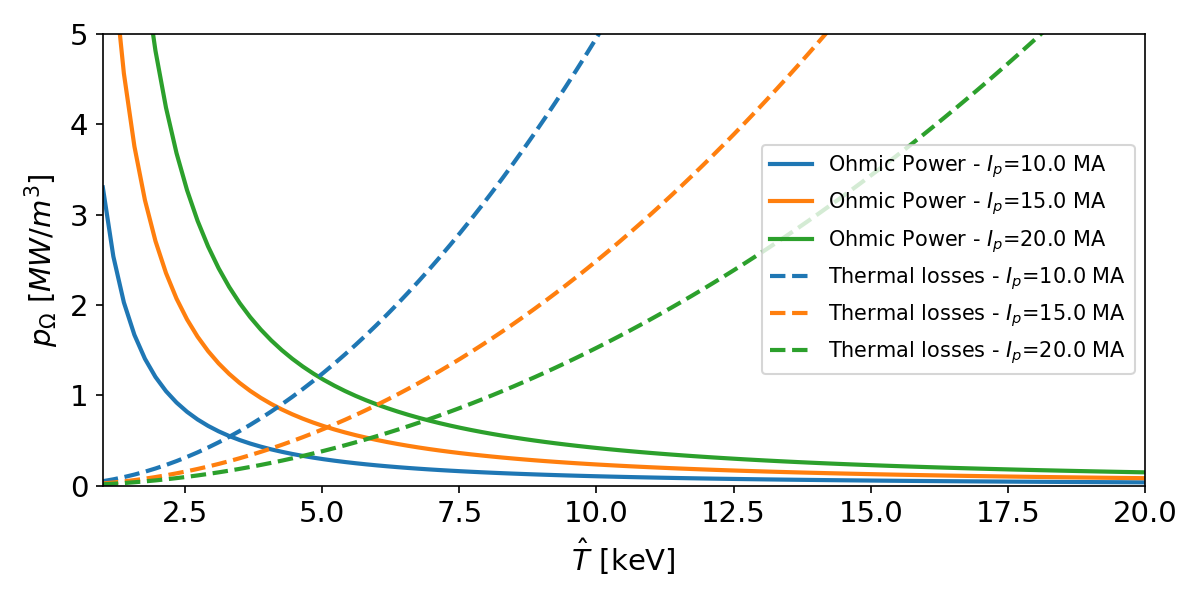
\includegraphics[width=1\linewidth]{figures/chap1/OhmicPower_vs_ThermalLosses}
	\caption{Ohmic Power Density and Thermal Losses as a function of the plasma temperature.}
	\label{fig:ohmicpowervsthermallosses}
\end{figure}

\subsection{The Need for Non-Inductive Current Drive}

Operating a tokamak in steady-state conditions means sustaining a constant current into plasma (Fig.\ref{fig:tokamak_transformer_effect}). However, inducing a constant plasma current requires ramping the current in the central solenoid, which can't be done indefinitely. The duration is limited by the magnetic flux (number of Volt-seconds) that can be provided by the central solenoid coil. So, tokamaks are intrinsically pulsed machines.
Thus, to run in steady-state, a tokamak requires the plasma current to be sustained by other non-inductive means, ie. "non-inductive" current drive. Current-drive methods such as by high-power radio waves also heat the plasma, but not all heating methods generate substantial plasma current density. 

\begin{marginfigure}[-3cm]
	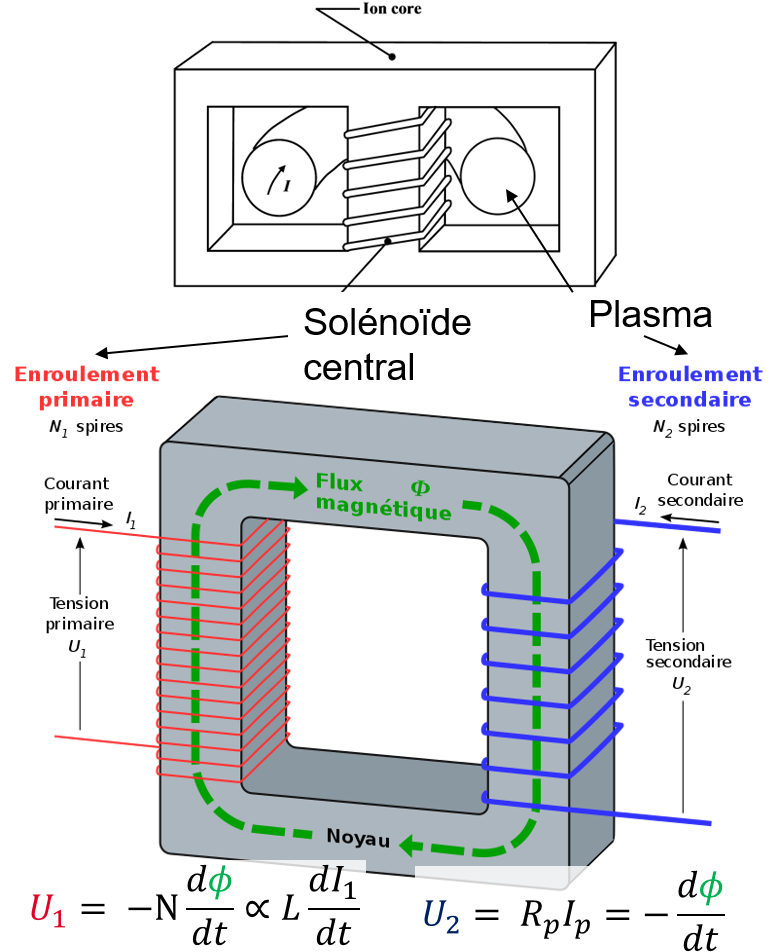
\includegraphics[width=1\linewidth]{figures/chap1/tokamak_transformer_effect}
	\caption{Tokamak transformer effect.}
	\label{fig:tokamak_transformer_effect}
\end{marginfigure}



\section{Radio frequency Heating and Current Drive}
\subsection{General Principles}
Radio-Frequency Heating and Current-Drive methods have in common the following systems:
\begin{itemize}
	\item Wave propagation and absorption on ions or electrons by wave-particle interactions
	\item Antennas to couple the electromagnetic power to plasma waves
	\item Transmission Lines to transport the electromagnetic power to the antennas
	\item High Power RF generators, that transform electrical power into electromagnetic power
\end{itemize}

The antenna coupling is 

we start from the lowest frequency range and continue to the highest



%%%%%%%%%%%%%%%%%%%%%%%%%%%%%%%%%%%%%%%%%%
\subsection{Ion Cyclotron Resonance Frequency}
\marginnote{Part of this chapter is taken from the chapter X of the IAEA Textbook of Fusion Technology [REF].}

\sidecite{kim2015}

%%%%%%%%%%%%%%%%%%%%%%%%%%%%%%%%%%%%%%%%%%
%%%%%%%%%%%%%%%%%%%%%%%%%%%%%%%%%%%%%%%%%%
\subsection{Lower Hybrid Resonance Frequency}
\marginnote{Part of this chapter is taken from the chapter X of the IAEA Textbook of Fusion Technology [REF].}
Originally, the occurrence of a wave resonance, the \emph{lower hybrid resonance}, has been anticipated to lead to strong wave-particle interaction through linear and non-linear mode conversion to a hot plasma wave\sidecite{stix1992}. With an appropriate RF launcher conceived to excite cold plasma waves, these would propagate into the plasma until reaching the lower hybrid resonant layer at $\omega_{LH}$. This resonance exists in tokamak plasma in the region close to the ion plasma frequency $\omega_{pi}/2\pi$, which lies in the lower end of the microwave band (1-5~GHz). At this layer, the perpendicular group velocity vanishes and the waves can convert into a hot plasma mode which is absorbed. This heating technique, known as \emph{Lower Hybrid plasma Ion Heating} (LHIH) or \emph{Lower Hybrid Resonance Heating} (LHRH), was the originally experimentally investigated method in the 70'\sidecite{bellan1974, hooke1972, golant1972, tonon1977}. Different physical mechanisms have been invoked to explain the energy absorption, such as stochastic Ion Heating in \citeauthyear{karney1978} and quasi-linear electron Landau damping in \citeauthyear{brambilla1983}.


In the 80', effective ion heating had only been obtained in a small number of experiments and research along the application of LH waves towards bulk ion heating were slowing down\sidecite{gormezano1986, porkolab1984, tonon1984}. The reason for this is that bulk ion heating near the mode conversion layer appeared to be less reproducible and more difficult to achieve than electron heating. Indeed, as the wave frequency gets closer to the lower hybrid frequency, the shorter wavelength waves may be more effectively absorbed and/or scattered near the plasma surface by non-linear effects such as parametric instabilities, low-frequency fluctuations, etc. Moreover, for LH bulk ion heating, the unconfined ions impinging on the wall induced a large amount of metallic impurities and then the increase of power radiated by the plasma.

Rather than trying to heat ions, it was theorized postulated that high phase velocity waves travelling in the direction parallel to the magnetic field could interact quasi-linearly by Landau interaction with the electrons population, and, by using an asymmetric spectrum could drive a large amount additional of toroidal plasma current \sidecite{fisch1978}. In the same fashion that for LHRH, the RF power is coupled to the plasma via launchers made of rectangular waveguides stacked periodically in the horizontal direction parallel to the toroïdal magnetic field. However, at the contrary of LHRH launchers, the LH waves are launched preferentially in one toroidal direction by mean of a phased array. The LH wave excited by such an array has an asymmetric parallel spectrum. The LH waves create an asymmetry in the electron distribution, which ultimately results in a net electric current \sidecite{fisch1987}. This technique is known as \emph{Lower Hybrid Current Drive} and despite the fact that the Lower Hybrid resonance is not any more involved in the use of this method in tokamaks, the term remained. LHCD has been confirmed on the PLT tokamak in 1982 \sidecite{bernabei1982} and in Alcator-C in 1984 \sidecite{porkolab1984}. 

Since in 1982 many impressive results were presented on LHCD\sidecite{stevens1983, porkolab1984, tonon1983} toward steady state or quasi steady state tokamak operations, most LH experiments were dedicated to electron interaction and especially to current drive. A recent review of LHCD is available in \sidecite{bonoli2014}.

Currently, the LH waves term refers to the waves which satisfy the slow-wave branch of the cold plasma dispersion relation for parallel index larger than one ($|n_{\parallel}|>1$) and a RF frequency $\omega$ which lies between the ion cyclotron $\omega_{ci}$ and the electron cyclotron $\omega_{ce}$ frequencies. 

%For the LH method which operates at the lower end of the microwave band (1-5 GHz) klystrons transform electrical power into electromagnetic power (step 1), which is transported to the plasma using waveguides (step 2). The power is coupled to the plasma with antennas called "grills" because of their characteristic shape (step 3), transported inside the plasma by plasma waves (typically the slow wave) (step 4), and absorbed on ions or electrons by wave-particle interaction (step 5).


\subsection{Klystrons}
A klystron is a vacuum tube used as amplifiers at narrow band microwave and radio frequencies. In the fusion domain, they are used mainly to produce high power waves, at the level of hundred of kilo watts during many seconds. First klystrons have been invented by the Varian brothers in 1937 \sidecite{Pond2008}. The first klystrons have been intensively used during World War II, as RF power generators for RADAR systems. Klystrons sources between 2.45 GHz and 5 GHz are now available at the 0.5-0.8 MW/10-1000 s level. 

\subsection{LH Transmission Lines}
As the RF frequency increases, coaxial cable losses (expressed in decibel per distance in Figure \ref{fig:rfcafetlattenuations}) become unpracticable for high power applications. In the LH range of frequencies (1-5 GHz), hollow rectangular waveguides are preferred for the transport of the RF power from the klystrons to the torus. In addition to their low losses, they also allow a greater breakdown voltage than coaxial lines of the same size. In this frequency range the wavelength in vacuum is of the order of 30 cm to 6 cm.


%\begin{figure}
%	\centering
%	\includegraphics[width=0.9\linewidth]{Figures/LHCD/RFCafe_TL_attenuations}
%	\caption{Various transmission line attenuation vs frequency. Source: \url{http://www.rfcafe.com/references/electrical/ew-radar-handbook/microwave-waveguide-coaxial-cable.htm}.}
%	\label{fig:rfcafetlattenuations}
%\end{figure}


\subsection{Rectangular waveguides} 
A hollow rectangular waveguide of width a and height b is illustrated in Figure \ref{fig:rectangularwaveguide}. Solving Maxwell’s equations for this geometry leads to multiple possible solutions, or \emph{modes}. These modes are eigenfunctions of the equation system. Each mode is characterized by a cut-off frequency, below which the mode cannot propagate in the guide. In a rectangular waveguide, modes can be expressed as \emph{Transverse Electric} (TE) or \emph{Transverse Magnetic} (TM), depending of their respective polarization. Since the walls of a rectangular waveguide constrain the electromagnetic field boundary conditions along two dimensions, two integer indices are used to describe a mode from another. Thus, modes in a rectangular waveguides can be $\mathrm{TE}_{10}$, $\mathrm{TE}_{20}$, $\mathrm{TM}_{11}$, etc. 

For practical applications, the dimensions of the waveguides are generally chosen in order to have one and only one mode allowed propagating for a specified frequency band. This single mode is the first one to appear to be propagating, and is referred as the \textit{fundamental mode} (generally labelled TE10). Other modes can eventually be excited by waveguides discontinuities, but can’t propagate since they are evanescent. They are referred to \textit{high order modes}.

For high power applications, a great care is given to waveguide inner walls, bends and connections, since reflected power and arcs may occur due to discontinuities in the conducting walls, such as the ones caused by misalignments, bumps, holes, etc.

%\begin{figure}
%	\centering
%	\includegraphics[width=0.5\linewidth]{Figures/LHCD/Rectangular_Waveguide}
%	\caption{Illustration of a rectangular hollow waveguide. Source:Wikipedia.}
%	\label{fig:rectangularwaveguide}
%\end{figure}


\subsection{Waveguide plumbery – a practical example with Tore Supra}
Many waveguide devices have been developed in order to transmit, measure, combine or split the power from one point to another. These devices are commonly used on LHCD systems to transport the power from a klystron to (a section of) an antenna, but also in order to protect the klystron from possible reflected RF power by the plasma.   

As an example of the usage of such devices, the Tore Supra LHCD system is illustrated in Figure \ref{fig:toresupralhcdsystem}. The power is generated at the klystron plant and transmitted to the two launchers through rectangular waveguides (8 lines per launcher). 

%\begin{figure}
%	\centering
%	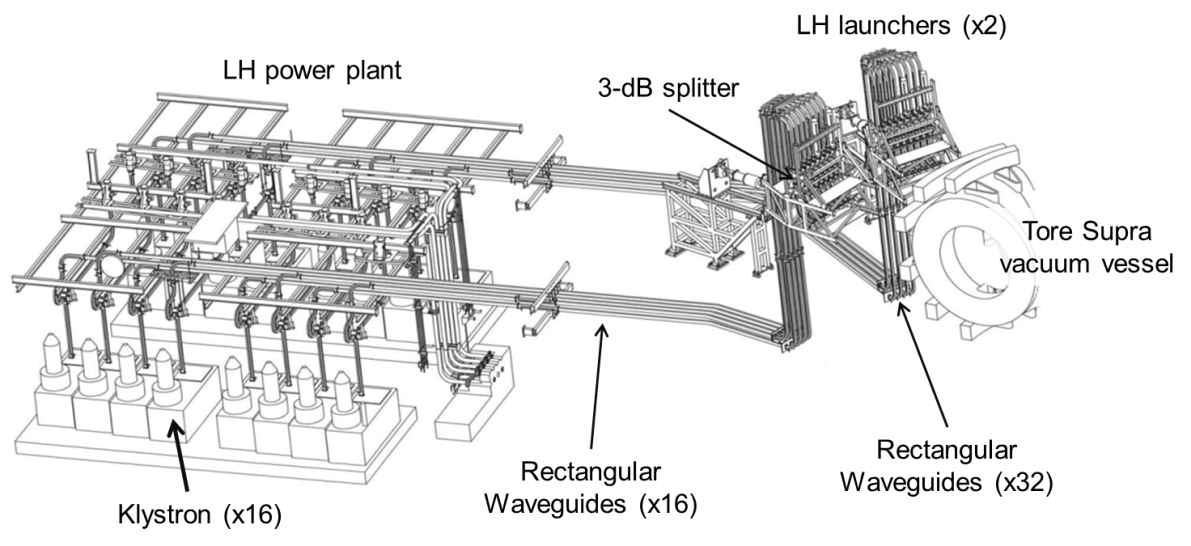
\includegraphics[width=0.9\linewidth]{Figures/LHCD/ToreSupra_LHCD_System}
%	\caption{Schematic of the Tore Supra LHCD system, from the klystrons plant to the vacuum vessel.}
%	\label{fig:toresupralhcdsystem}
%\end{figure}


Once reaching the launcher rear end, the power goes trough a \textit{hybrid junction} (also called 3-dB splitter). This device splits the incident power into two waveguides, one to feed the upper part and the other for the lower part of the launcher.  If reflected power (from the plasma) returns from these two waveguides, the power is recombined and directed to a fourth one. An actively cooled water load is connected to this fourth port, in order to dump the remaining RF power reflected by the plasma and thus protect the klystron. A rectangular waveguide 3-dB splitter is illustrated in Figure \ref{fig:hybridjunction1}. 

%\begin{figure}
%	\centering
%	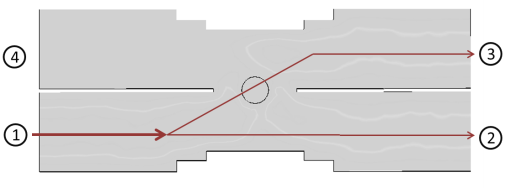
\includegraphics[width=0.4\linewidth]{Figures/LHCD/HybridJunction1}
%	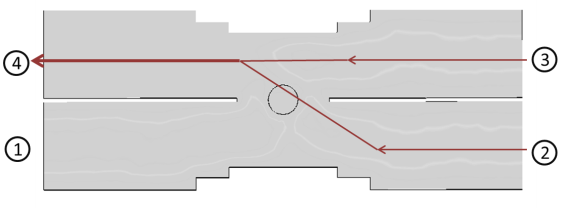
\includegraphics[width=0.4\linewidth]{Figures/LHCD/HybridJunction2}
%	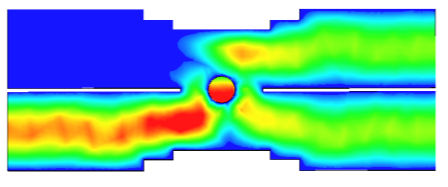
\includegraphics[width=0.4\linewidth]{Figures/LHCD/HybridJunction_Efield}
%	\caption{Top: Illustration of an rectangular waveguide hybrid junction. When excited from port 1, the power is split to ports 2 and 3. when the power comes from ports 2 and 3, the power is recombined and directed to port 4, where the power is dumped into a water load. Bottom: The electric field distribution when excited from port 1. }
%	\label{fig:hybridjunction1}
%\end{figure}


After being split, the RF power goes through various devices up to the plasma (Figure \ref{fig:toresuprac4cad}): 
\begin{itemize}
	\item A bidirectional coupler, which allows measuring the forward and reflected power amplitude and phase ;
	\item A DC break, which isolates the DC potential of the tokamak from the DC potential of the transmission line (for the protection of persons);
	\item A vacuum feed through (window) which isolates the tokamak vacuum from the pressurized medium existing in the waveguide. These windows (16 by launchers) are illustrated in Figure \ref{fig:toresuprac4cad}. A window consists in a dielectric medium inserted between two rectangular waveguides. The dimensions of the dielectric medium (a ceramic, such beryllium oxide BeO or alumina) are calculated in order not producing reflected power. A part of the power is always absorbed in the ceramic, so a great care is applied to correctly cool the window in order to avoid heating up and ultimately break the ceramic.
	\item A TE10-TE30 mode converter, which splits the incoming RF power into three, thus leading to split the power into three poloidal rows of waveguides. A mode converter is a rectangular waveguide device which large side is modulated in order to allow higher modes (such as TE20, TE30 and TE40) and such that the power is totally transferred from one mode to another one (efficiency is close to 100\%). Once the power is transferred to the TE30 mode, metallic septa located in zero field regions split the power into three independent waveguides. The device is illustrated in Figure \ref{fig:modeconverter}.
	\item Finally a multijunction, a structure which will be described in details in the next section, splits and phases the power in the toroidal direction, then leads to the plasma. 
\end{itemize}


%\begin{figure}
%	\centering
%	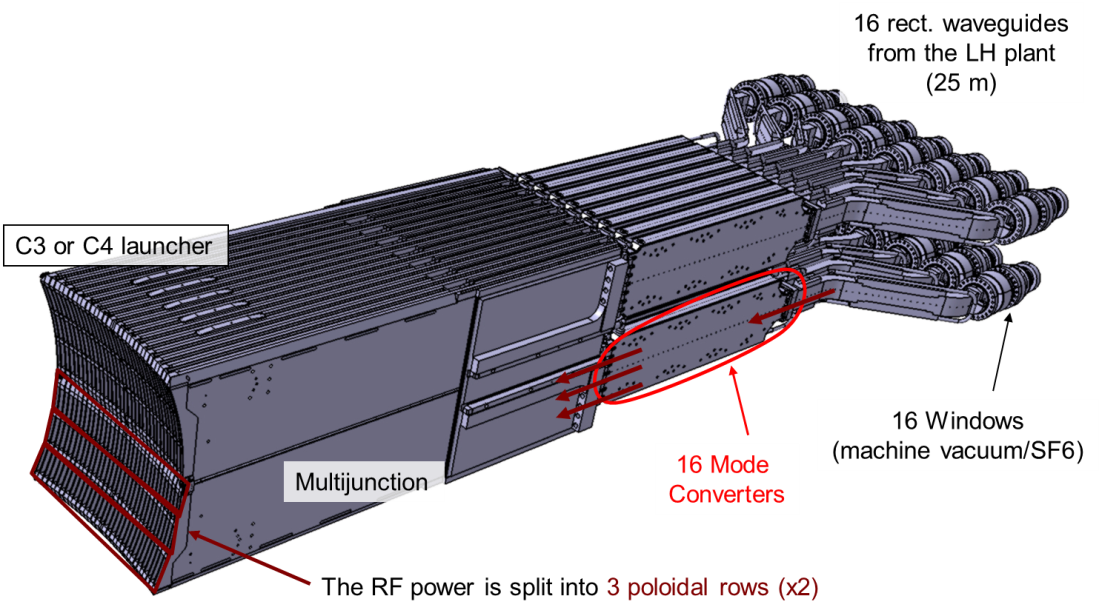
\includegraphics[width=0.9\linewidth]{Figures/LHCD/ToreSupra_C4_CAD}
%	\caption{Illustration of the power splitting scheme in Tore Supra LHCD launcher C3 or C4.}
%	\label{fig:toresuprac4cad}
%\end{figure}
%
%
%\begin{figure}
%	\centering
%	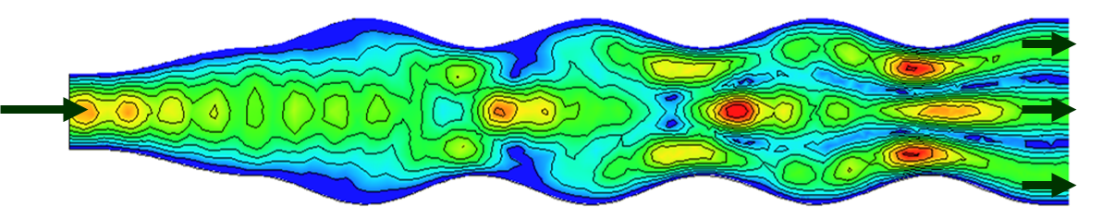
\includegraphics[width=0.9\linewidth]{Figures/LHCD/ModeConverter}
%	\caption{Illustration of the electric field distribution in a TE10-TE30 mode converter at 5 GHz. The device is excited from the left.}
%	\label{fig:modeconverter}
%\end{figure}
